% Chapter Template

\chapter{Methods} % Main chapter title
\label{ChapterX} % Change X to a consecutive number; for referencing this chapter elsewhere, use \ref{ChapterX}



%----------------------------------------------------------------------------------------
%	SECTION 1
%----------------------------------------------------------------------------------------

\section{A new approach to track intracerebral bloodflow}
Typically GCaMP signals are recorded at a sampling rate of 25Hz \parencite{celotto2020analysis}. In contrast the dataset at hand was recorded at 100Hz. Highspeed recordings bear potentials for the analysis of neural signals beyond the frequency of neocortical slow waves. However, new methods must be established to identify what high frequency components relate to. This is especially important because widefield flouroscence recordings are confounded with an error that results from the hemodynamic autoflourescence. The results of a new approach indicate that high high frequencies in the df/f signal relate to particles of hemoglobin rich blood that flow through intracerebral bloodvessels of various size.\\
\begin{figure}[th]
\centering
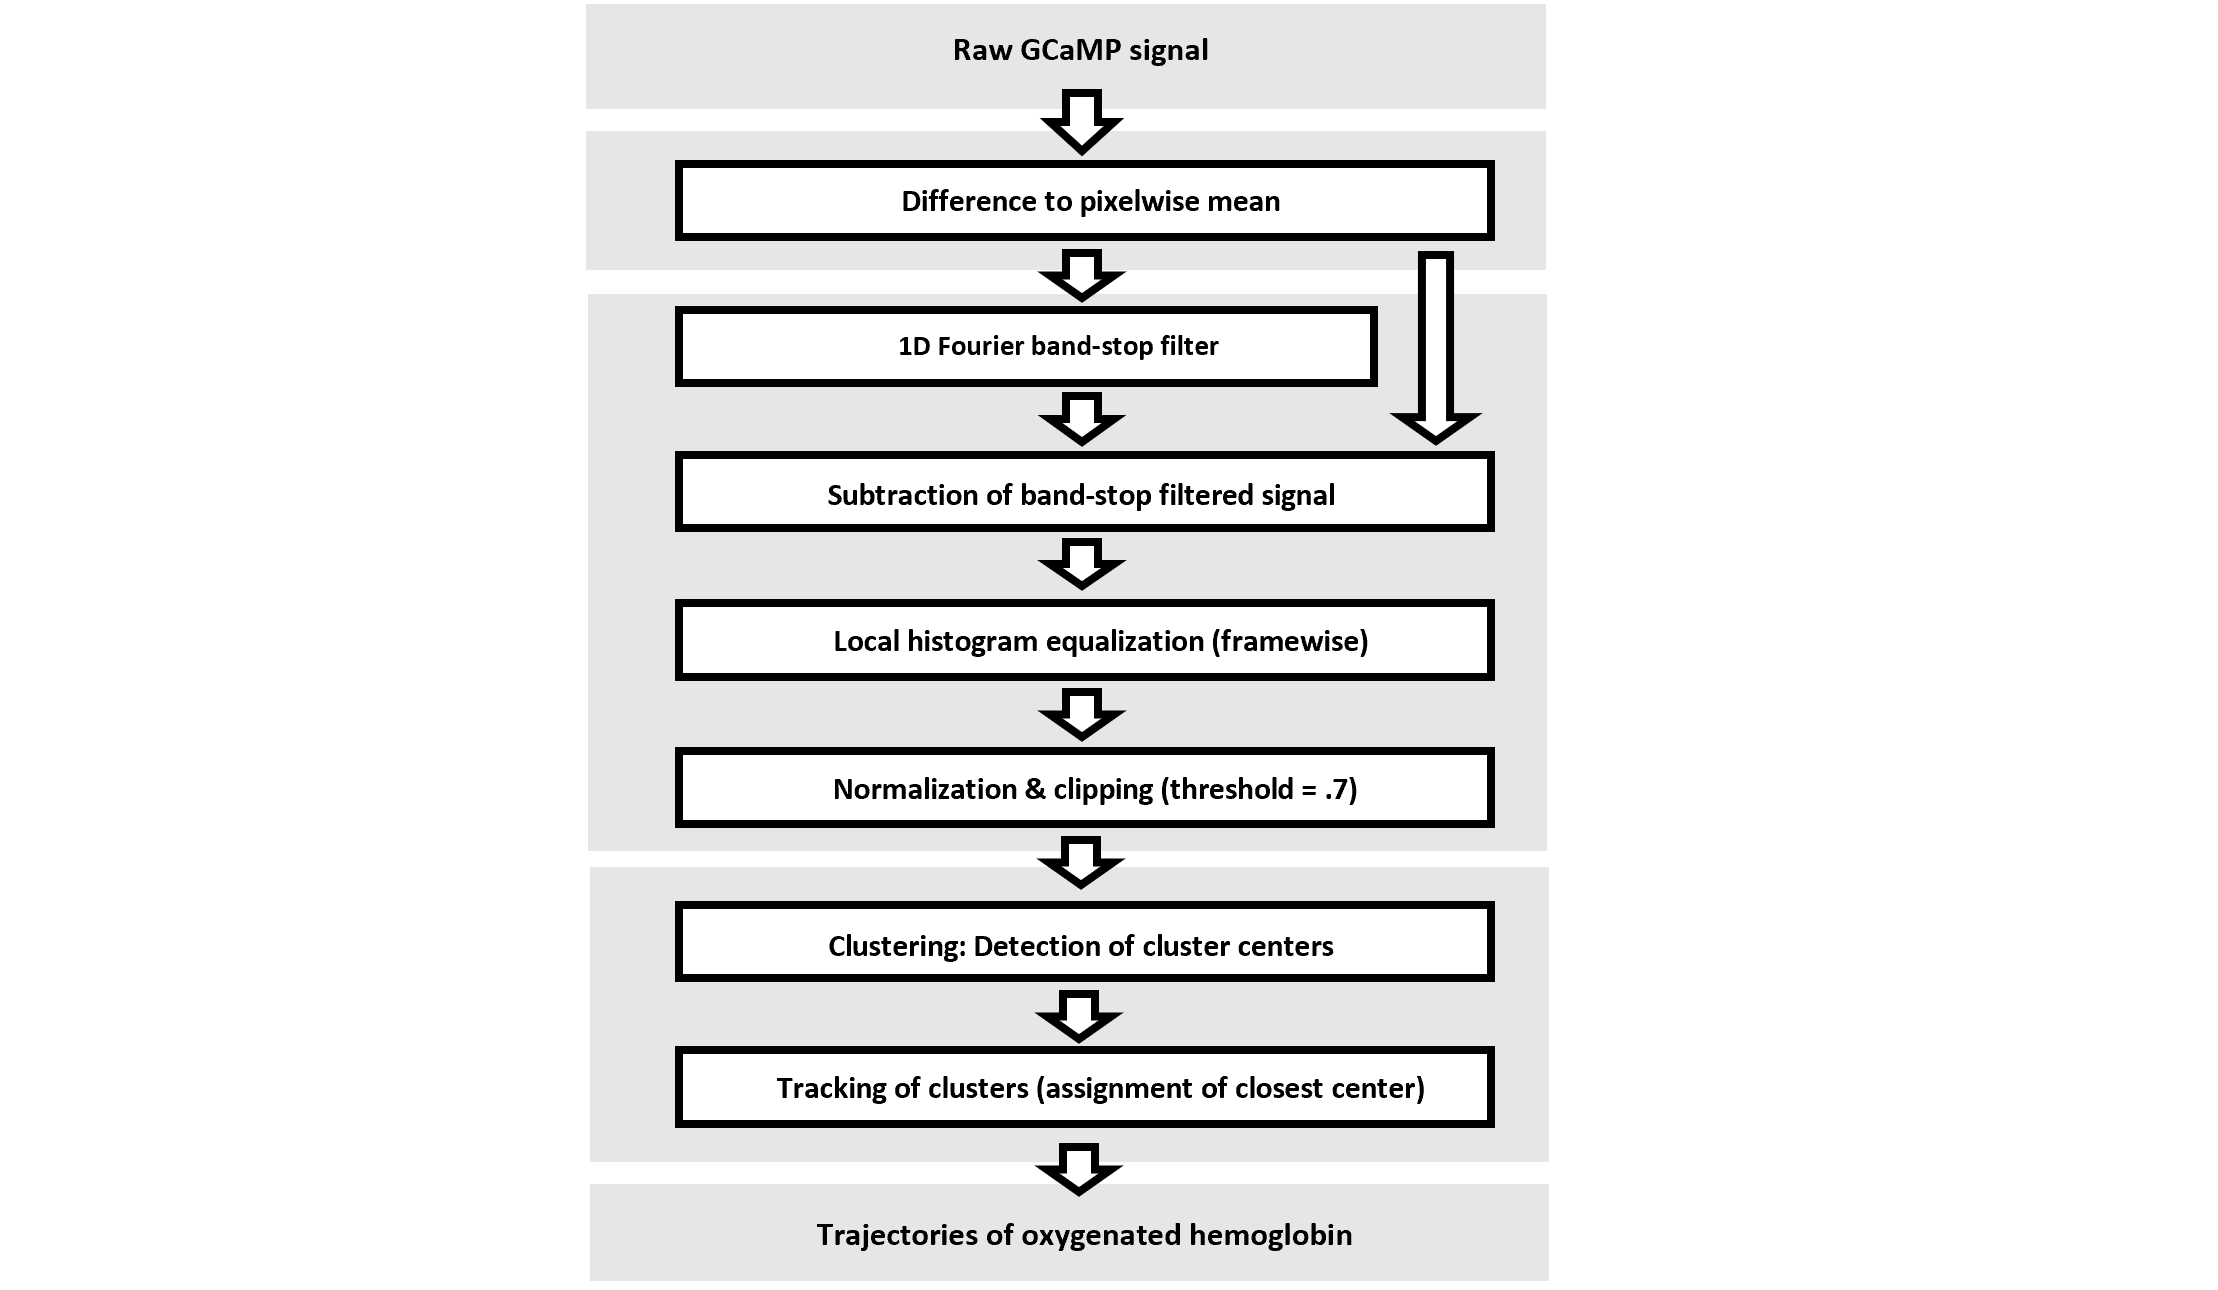
\includegraphics[width=\textwidth,height=\textheight,keepaspectratio]{Figures/tracking_bloodflow_pipeline}
\decoRule
\caption[Processing pipeline for the detection of bloodflow]{Processing pipeline for the detection of bloodflow}
\label{fig:clustering_approach_pipeline}
\end{figure}
\begin{figure}[th]
\centering
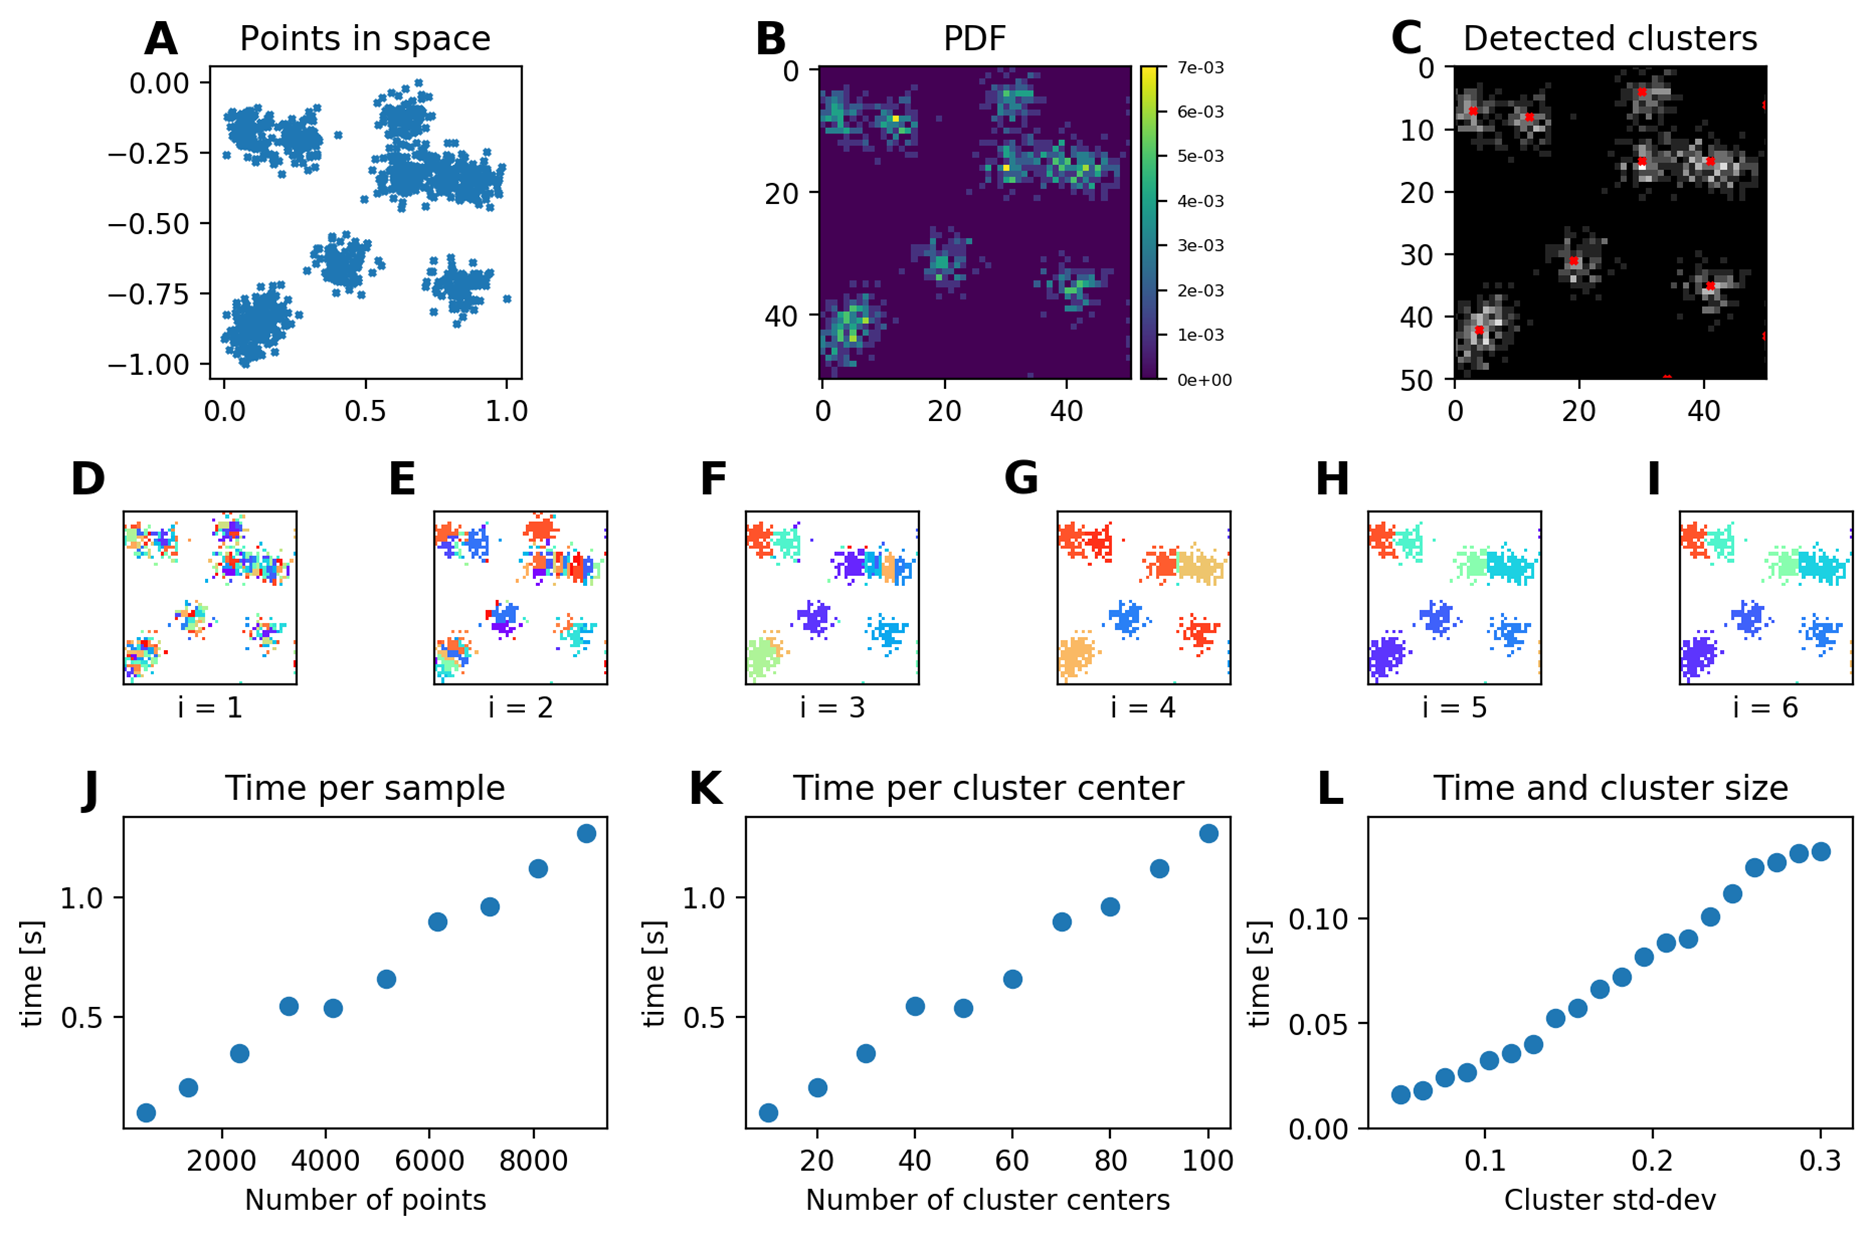
\includegraphics[width=\textwidth,height=\textheight,keepaspectratio]{Figures/clustering_approach_properties}
\decoRule
\caption[A mean shift approach for clustering pixels]{A mean shift approach for clustering pixels. After clipping the preprocessed hemodynamic signal, groups of bright, rather isolated foreground pixels are visible. These pixels can be considered as evidence for the presence of oxygenated hemoglobin particles. To detect the location of named clusters of pixels a variation of mean shift clustering was implemented that works with density matrices. Panel A: A distribution of points in $\mathbb{R^2}$. Cluster centers were sampled using a 2D gaussian. For each cluster center points were added using a second gaussian probability distribution centered at the respective location. Panel B : A 2D histogram of the distibution in panel A indicating the probability density function. Panel C: The detected cluster centers. Panels D-E: Assignment of pixels to clusters for the first seven iterations beginning with i=1. After iteration seven convergence is achieved. Panel J: Time per sample. Panel K: Time per cluster Panel L: Time per cluster size. }
\label{fig:clustering_approach_properties}
\end{figure}
\begin{figure}[th]
\centering
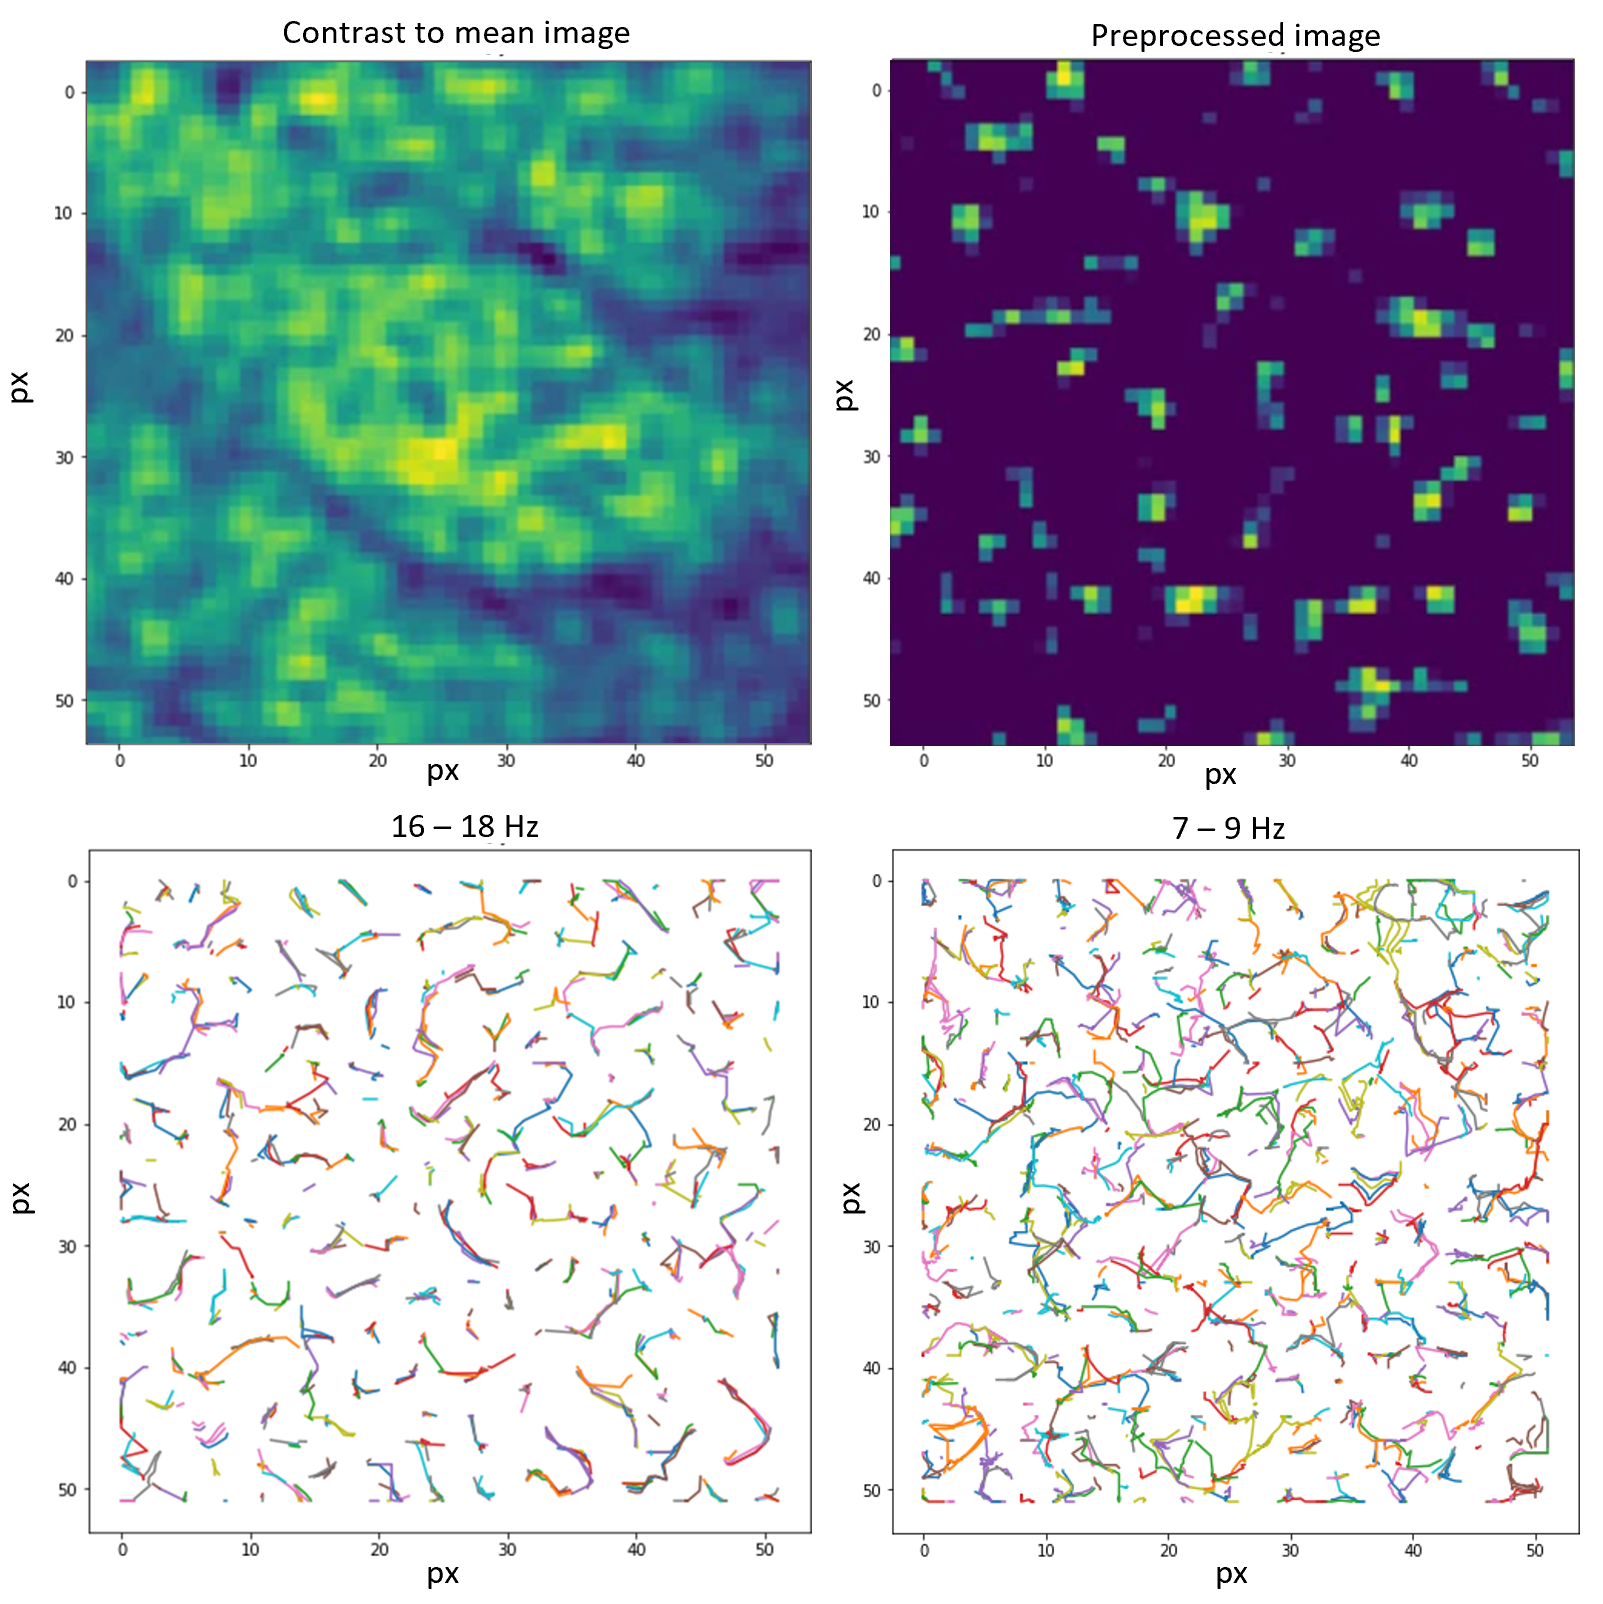
\includegraphics[width=\textwidth,height=\textheight,keepaspectratio]{Figures/clustering_approach_results}
\decoRule
\caption[Cluster tracking reveals trajectories of oxygenated hemoglobin]{Cluster tracking reveals trajectories of oxygenated hemoglobin.\\
Upper left: A sample frame for the original contrast to the pixelwise mean. Upper right: The preprocessed frame after application of clipping. Lower left: Detected trajectories for filtering of frequencies in the range of the heartbeat. Lower right: Detected trajectories of bloodflow for filtering of low frequencies. See also figure \ref{fig:clustering_approach_properties}}
\label{fig:clustering_approach_results}
\end{figure}
The approach presented here allows to measure intracerebral bloodflow without the need for the injection of tracers. Typically, microbeads are used to detect the flow rates and speed of intracerebral blood \parencite{kim2019development}. The study of intracranial bloodflow bears potentials for a better understanding of pathologic conditions and basic neurobiological functions of the brain. For example it was shown that the microvessel density decreases in brain tumors and characteristic chnages in the hemoglobin concentration can be observed \parencite{lee2014vivo}. However intracerebral bloodflow is also addressed in the neuroscience in the study of neurometabolic and neurovascular coupling \parencite{devor2012frontiers}. New approaches to track the bloodflow in the brain could help to better understand the interaction between the activity of neurons and bloodflow.\\
To determine what high frequency components of the flourescence signal relate to several processing steps were employed (see \ref{clustering_approach_pipeline}). First the mean image was calculated and subtracted from each frame of the recorded videos. The signal in time for each pixel was then bandstop filtered and the difference to the original signal was calculated. Bandstop filtering was achieved by tranforming the vectors to the fourier domain and setting the frequency components in the desired range to zero before applying inverse fourier transform. Adaptive histogram equalization was used to improve the contrast of each frame after clipping all values below a given threshold. In the resulting videos clusters of bright foreground pixels move on decisive trajectories (see figure \ref{fig:clustering_approach_results}).\\
Cluster tracking is used to measure the pathways of these temporospatial patterns. Objects in binary images that are potentially connected are oftenly labeled using watershed distance transform \parencite{arganda-carreras2016distance} \footnote{Distance transform assigns the value to the closest background pixel to each foreground pixel. Different algorithms exist that allow for fast approximations. The resulting image represents a heightmap if the distance values are interpreted as depth. A simple flooding algorithm can be used to determine the watersheds: A simulated rise of the water level fills basins in the heightmap. The borders between adjecent basins are the watersheds that seperate the detected objects.}. As the data was (1) not binarized but clipping was used and (2) has a low relative resolution which results in a rough outline does not allow for the computation of meaningful watersheds a different approach was used to detect clusters of connected foreground pixels. This approach represents a mean shift technique. \\
The clipped images were interpreted as probability density functions that indicate the presence of oxygenated hemoglobin. Clusters are detected by iteratively moving the density at a given location towards the center of gravity of a patch around this location. The algorithm stops if convergence is achieved or a maximal number of iterations is reached. The environment could be a squre or a circular patch. The impact could be weigthed using a 2D gaussian kernel to reduce the impact of distant points on the center of gravity. For the results shown in figure \ref{fig:clustering_approach_results} a simple rectangular patch was used. \\
Important properties were studied with simulated data. Figure \ref{fig:clustering_approach_properties} summarizes the results. The computation of 2D histograms can be achieved in o(n) as iterating over the data once is sufficient. As the size of this histogram can be chosen freely the computatio time does not directly depend on the number of samples. In the simulation data for each cluster was sampled using the same 2D gaussian with a given standard deviation. Given that convergence can be achieved it can hence be assumed that in average the algorithm takes the same amount of time for each cluster. The simulation confirmed a linear relationship (\ref{fig:clustering_approach_properties}K). Increasing the number of samples per cluster center also scales linearly with the processing time. A different picture shows for variations of the standard deviation of the cluster centers. A nonlinear relationship can be assumed.\\
Clustering was performed for each frame seperately. Tracking was achieved by assigning the closest cluster center of the subsequent frame (maximal distance 10 px). It shows that particles move on decisive trajectories. Deviant results can be achieved for different frequencies. If bandstop filtering is applied in the range of the heart rate shorter trajectories are detected. The clusters appeared to be larger indicating bloodflow in bigger vessels. In contrast for smaller vessels a more filigree pattern can be observed. It can be hypothesized that these patterns relate to blood that travels at different speeds in vessels of different size.

%----------------------------------------------------------------------------------------
%	SECTION 1
%----------------------------------------------------------------------------------------
\section{Dense Optical Flow}

Lorem ipsum dolor sit amet, consectetur adipiscing elit. Aliquam ultricies lacinia euismod. Nam tempus risus in dolor rhoncus in interdum enim tincidunt. Donec vel nunc neque. In condimentum ullamcorper quam non consequat. Fusce sagittis tempor feugiat. Fusce magna erat, molestie eu convallis ut, tempus sed arcu. Quisque molestie, ante a tincidunt ullamcorper, sapien enim dignissim lacus, in semper nibh erat lobortis purus. Integer dapibus ligula ac risus convallis pellentesque.

\section{Helmholtz-Decomposition}

\section{Helmholtz-Decomposition of Dense Optical Flow}

\section{The processing pipeline}
Widefield flouroscence microscopy makes use of slective differences in the reflectance of light of a specific wavelength that results from conformational changes of ion channels in the neural membrane. This approach is challanged by the hemodynamic autoflourescence due to the blood oxygen level. The flouroscence of oxygenated and deoxigenated hemoglobin depends on the frequency of the light used for illumination. At a wavelength of 405nm the differences are marginal. Nonetheless a hemodynamic error signal remains in the data. Fluctuations are especially visible in recordings with 100 Hz sampling rate as it is high enough to capture potential fluctuations in the flourescence due to breathing and the heartbeat. This is especially relevant for for deep anaesthesia as the GCaMP signal to hemodynamic noise ratio is higher.\\
